\documentclass{article}
\usepackage[utf8]{inputenc}
\usepackage[spanish]{babel}
\usepackage{listings}
\usepackage{subfigure}
\usepackage{graphicx}
\usepackage{url}
\usepackage{multirow}
\usepackage{color}
\usepackage{booktabs}
\usepackage{float}
\usepackage{hyperref}
\usepackage[margin=3cm,twoside]{geometry} 
\setlength{\parindent}{0pt}
\setlength{\parskip}{1em}


\definecolor{mygreen}{rgb}{0,0.6,0}
\definecolor{mygray}{rgb}{0.5,0.5,0.5}
\definecolor{mymauve}{rgb}{0.58,0,0.82}
\lstset{ 
  backgroundcolor=\color{white},   % choose the background color; you must add \usepackage{color} or \usepackage{xcolor}; should come as last argument
  basicstyle=\footnotesize,        % the size of the fonts that are used for the code
  breakatwhitespace=false,         % sets if automatic breaks should only happen at whitespace
  breaklines=true,                 % sets automatic line breaking
  captionpos=b,                    % sets the caption-position to bottom
  commentstyle=\color{mygreen},    % comment style
  deletekeywords={...},            % if you want to delete keywords from the given language
  escapeinside={\%}{)},          % if you want to add LaTeX within your code
  extendedchars=true,              % lets you use non-ASCII characters; for 8-bits encodings only, does not work with UTF-8
  firstnumber=1,                % start line enumeration with line 1000
  frame=single,	                   % adds a frame around the code
  keepspaces=true,                 % keeps spaces in text, useful for keeping indentation of code (possibly needs columns=flexible)
  keywordstyle=\color{blue},       % keyword style
  language=Octave,                 % the language of the code
  morekeywords={*,...},            % if you want to add more keywords to the set
  numbers=left,                    % where to put the line-numbers; possible values are (none, left, right)
  numbersep=5pt,                   % how far the line-numbers are from the code
  numberstyle=\tiny\color{mygray}, % the style that is used for the line-numbers
  rulecolor=\color{black},         % if not set, the frame-color may be changed on line-breaks within not-black text (e.g. comments (green here))
  showspaces=false,                % show spaces everywhere adding particular underscores; it overrides 'showstringspaces'
  showstringspaces=false,          % underline spaces within strings only
  showtabs=false,                  % show tabs within strings adding particular underscores
  stepnumber=1,                    % the step between two line-numbers. If it's 1, each line will be numbered
  stringstyle=\color{mymauve},     % string literal style
  tabsize=2,	                   % sets default tabsize to 2 spaces
  title=\lstname                  % show the filename of files included with \lstinputlisting; also try caption instead of title
}
\usepackage{etoolbox}
\makeatletter
\providecommand{\subtitle}[1]{% add subtitle to \maketitle
  \apptocmd{\@title}{\par {\large #1 \par}}{}{}
}
\makeatother
\title{Tarea 2 de Modelos Probabilistas Aplicados}
\subtitle{Frecuencias y histogramas}

\author{5271}
\date{\today}

\begin{document}

\maketitle

\section{Origen de los datos}

En este trabajo se utilizo como fuente de los datos el libro ``The Adventures of Sherlock Holmes", del escritor y médico británico Arthur Conan Doyle. Este libro se encuentra disponible en la biblioteca virtual gratuita Project Gutenberg, al que se puede acceder desde el siguiente enlace: \href{https://www.gutenberg.org}{https://www.gutenberg.org}. 

\section{Sobre el libro}

Este libro es una colección de doce cuentos de Arthur Conan Doyle , los cuales fueron publicados por primera vez el 14 de octubre de 1892. El mismo agrupa los primeros cuentos con el detective consultor Sherlock Holmes , que se habían publicado en doce números mensuales de The Strand Magazine de Julio de 1891 a junio de 1892. 

\section{Análisis y tratamiento de los datos}

Al libro seleccionado se le realiza un estudio de frecuencia de ocurrencia tanto de las letras como de las palabras que compone el texto. El análisis será realizado en el programa R versión 4.0.2 \cite{r} en el entorno de desarrollo Rstudio \cite{rstudio}. 

\subsection{Letras}
De le libro en cuestión se extrajeron todas las letras que componen el texto, teniendo el mismo $432064$ caracteres alfanuméricos que fueron almacenados en un \textit{Data frame}, como se muestra en el cuadro \ref{tab:1} de la página \pageref{tab:1}. De los datos obtenidos solo necesitamos las letras por lo cual procedemos a un filtrado del \textit{Data frame}. A partir de los datos filtrados se realiza un análisis de frecuencia de ocurrencia de las letras en el texto, como se muestra en el cuadro \ref{tab:2} de la página \pageref{tab:2}. Para una mejor comprensión de los datos obtenidos se realiza una representación gráfica de los mismos mediante un histograma, como se puede observar en la figura  \ref{fig:1} de la página \pageref{fig:1}

% Table generated by Excel2LaTeX from sheet 'Hoja1'
\begin{table}
  \centering
  \caption{fragmento del \textit{Data frame} que contiene todos los caracteres que aparecen en el texto. }
    \begin{tabular}{ccc}
    \toprule
          & \textbf{gutenberg\_id} & \textbf{letra} \\
    \midrule
    1     & 1661  & t \\
    2     & 1661  & h \\
    3     & 1661  & e \\
    4     & 1661  & a \\
    5     & 1661  & d \\
    6     & 1661  & v \\
    7     & 1661  & e \\
    8     & 1661  & n \\
    9     & 1661  & t \\
    10    & 1661  & u \\
    \bottomrule
    \end{tabular}%
  \label{tab:1}%
\end{table}%
% Table generated by Excel2LaTeX from sheet 'Hoja1'
\begin{table}
  \centering
  \caption{fragmento de \textit{Data frame} que contiene la frecuencia de ocurrencia de cada letra en el texto}
    \begin{tabular}{ccr}
    \toprule
          & \textbf{Var1} & \multicolumn{1}{c}{\textbf{Freq}} \\
    \midrule
    11    & a     & 35137 \\
    12    & b     & 6362 \\
    13    & c     & 10499 \\
    14    & d     & 18563 \\
    15    & e     & 53111 \\
    16    & f     & 8975 \\
    17    & g     & 7887 \\
    18    & h     & 29047 \\
    19    & i     & 30140 \\
    20    & j     & 452 \\
    21    & k     & 3543 \\
    22    & l     & 17145 \\
    23    & m     & 11787 \\
    \bottomrule
    \end{tabular}%
  \label{tab:2}%
\end{table}%

\begin{figure}
\centering
\subfigure[Frecuencia de ocurrencia de las letras en el texto]{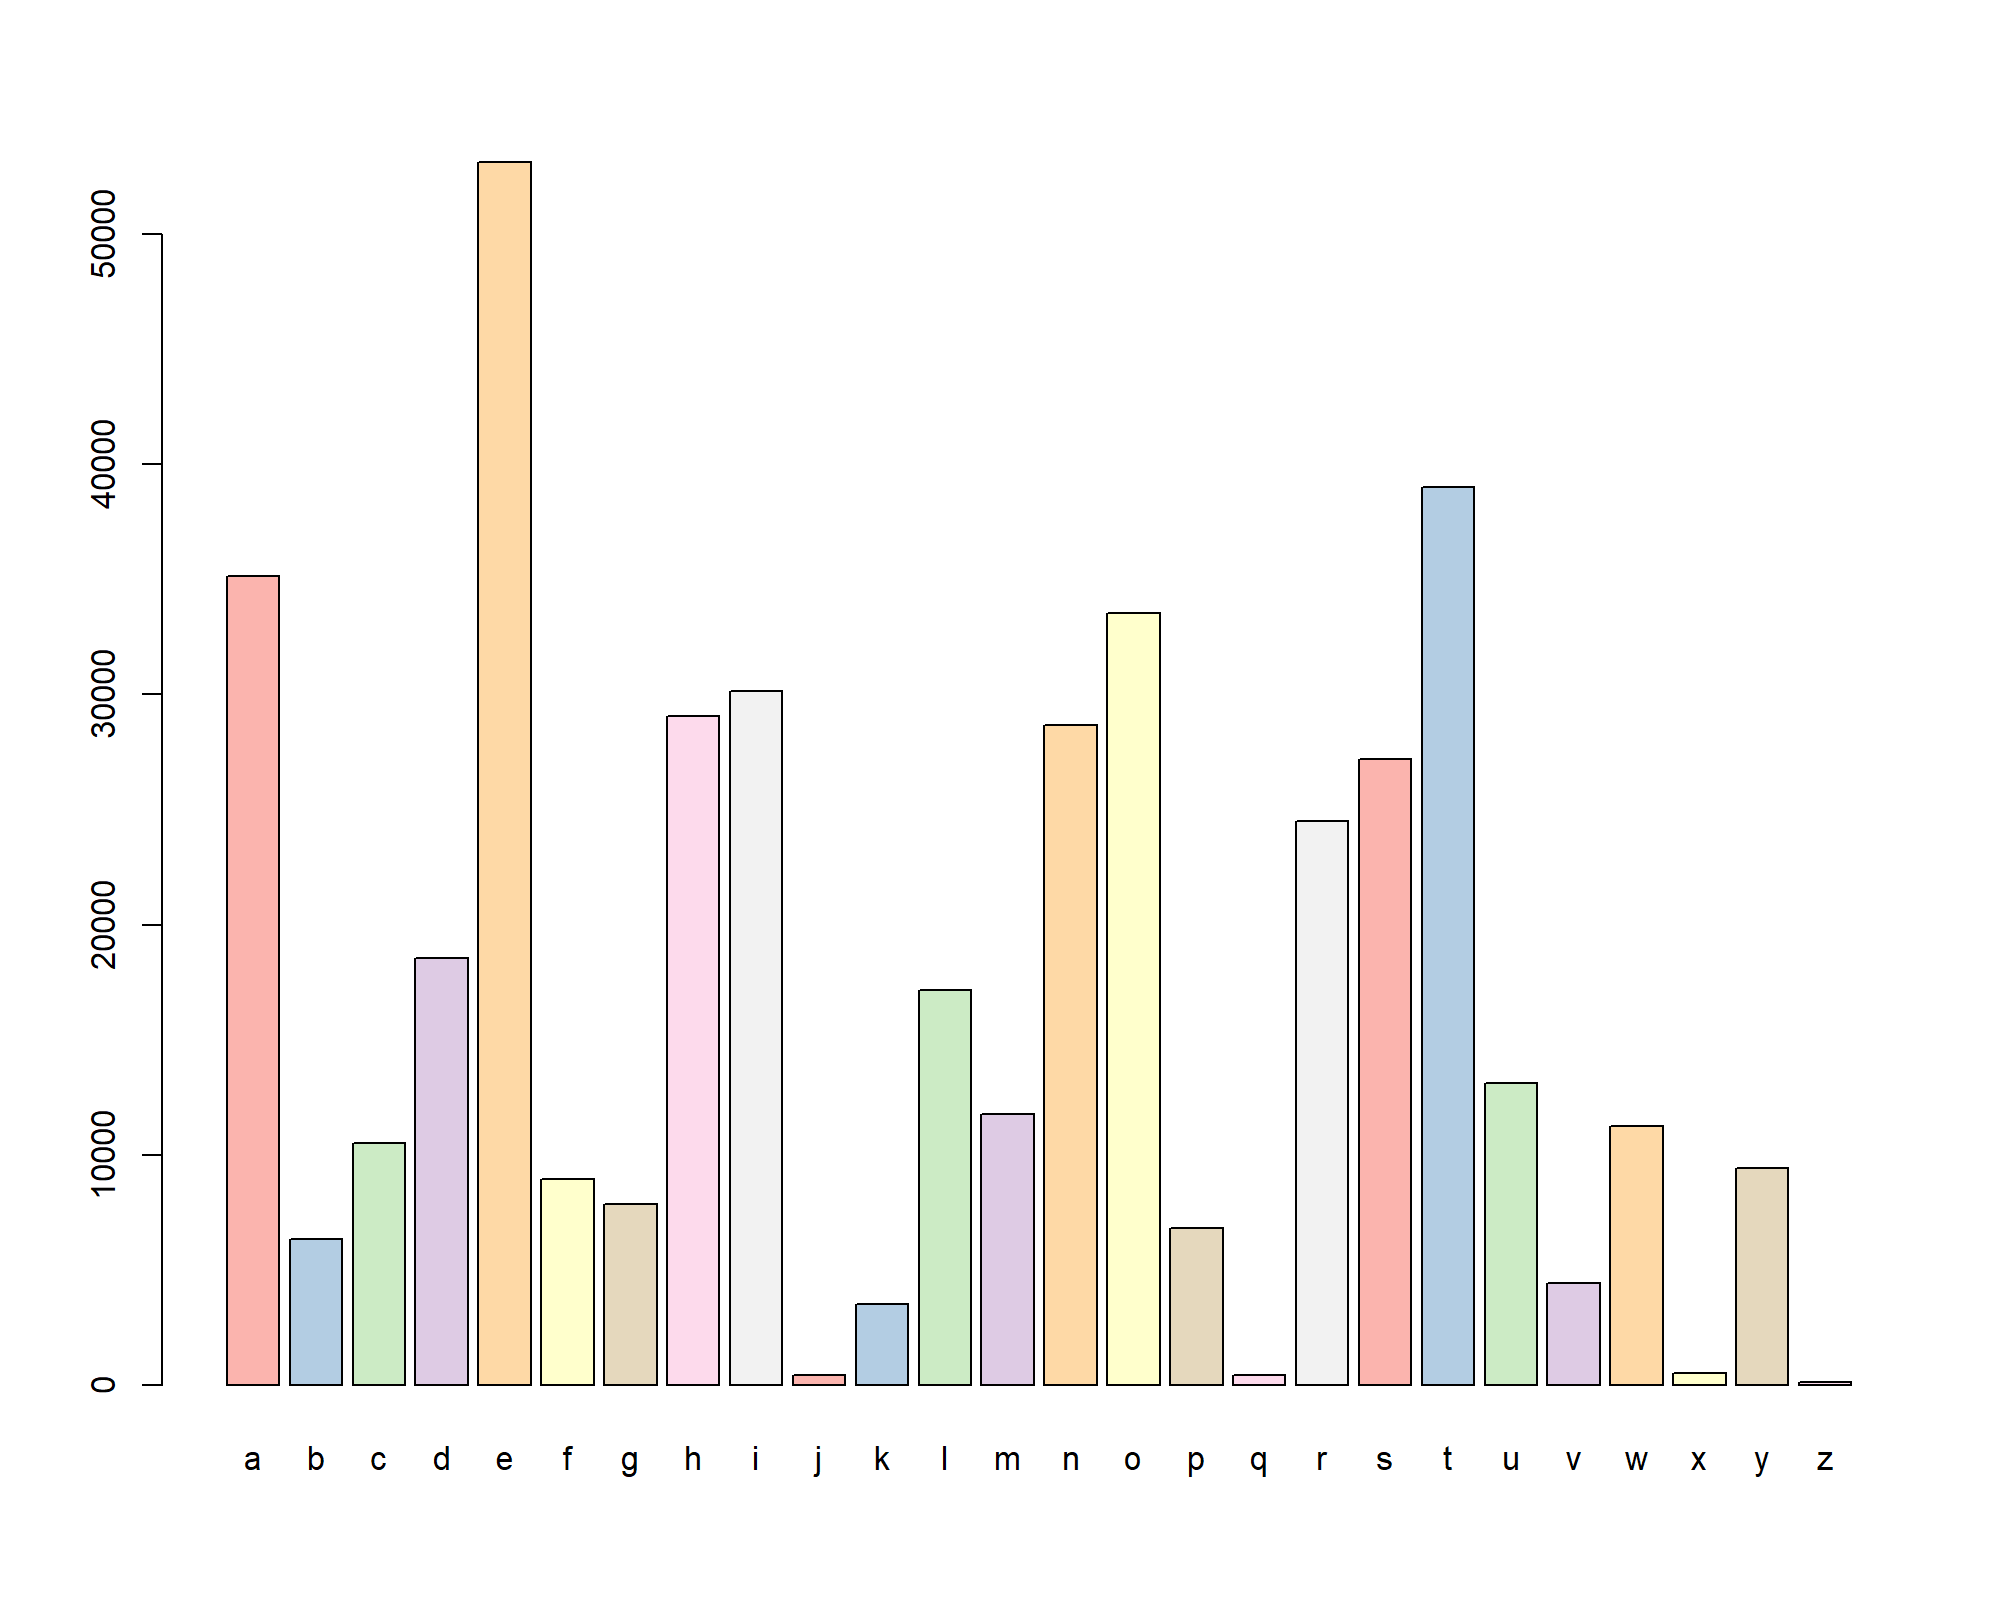
\includegraphics[scale=0.5]{figuras/frecuencialetras.png}}
\subfigure[Frecuencia de ocurrencia de las letras en el texto ordenada de manera decreciente]{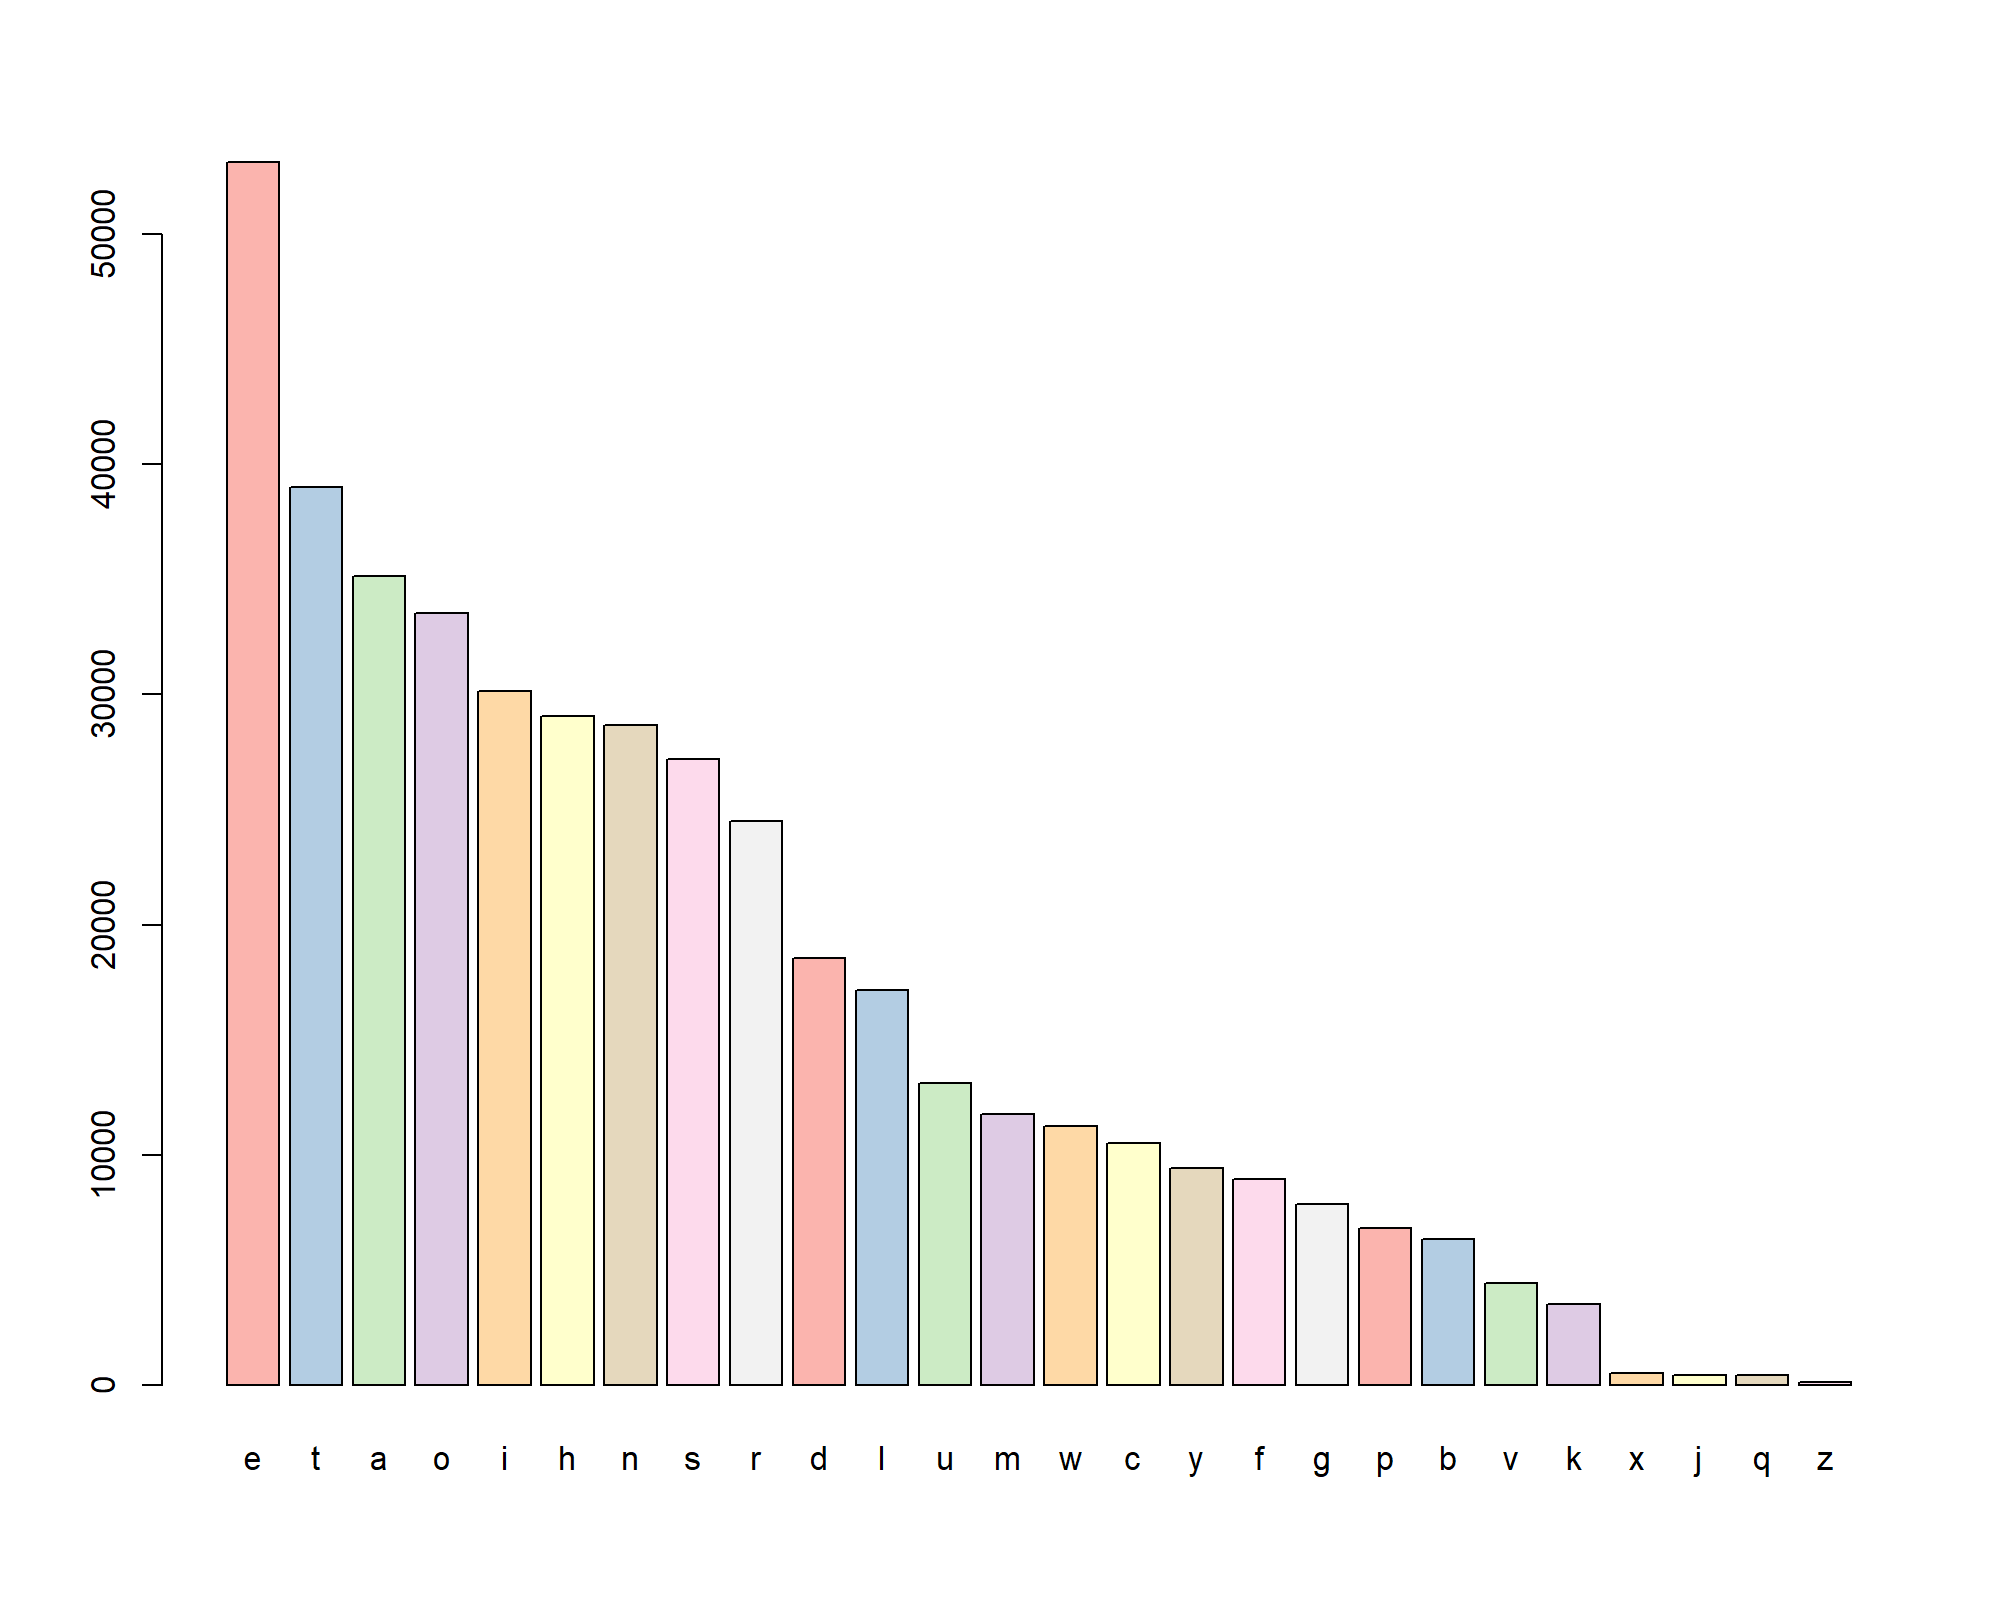
\includegraphics[scale=0.5]{figuras/frecuencialetrasdecres.png}}
\caption{Histogramas de frecuencia de ocurrencia de las letras en el texto}
\label{fig:1} 
\end{figure}
 


 \subsection{Palabras}
 Para el trabajo con las palabras, se extraen todas las presentes en el texto, teniendo el mismo $432064$ palabras que fueron almacenadas en un \textit{Data frame}, como se muestra en el cuadro \ref{tab:3} de la página \pageref{tab:3}. A partir de los datos obtenidos se realiza un análisis de frecuencia de ocurrencia de las palabras en el texto, como se muestra en el cuadro \ref{tab:4} de la página \pageref{tab:4}. Para una mejor comprensión de los datos obtenidos se realiza una representación gráfica de los mismos mediante un histograma, como se puede observar en la figura  \ref{fig:2} de la página \pageref{fig:2}
 
 % Table generated by Excel2LaTeX from sheet 'Hoja1'
\begin{table}
  \centering
  \caption{fragmento del \textit{Data frame} que contiene todas las palabras que aparecen en el texto.}
    \begin{tabular}{ccl}
    \toprule
          & \textbf{Gutenberg\_id} & \textbf{Palabra} \\
    \midrule
    1     & 1661  & the \\
    2     & 1661  & adventures \\
    3     & 1661  & of \\
    4     & 1661  & sherlock \\
    5     & 1661  & holmes \\
    6     & 1661  & by \\
    7     & 1661  & sir \\
    8     & 1661  & arthur \\
    9     & 1661  & conan \\
    10    & 1661  & doyle \\
    \bottomrule
    \end{tabular}%
  \label{tab:3}%
\end{table}%
% Table generated by Excel2LaTeX from sheet 'Hoja1'
\begin{table}
  \centering
  \caption{fragmento de \textit{Data frame} que contiene la frecuencia de ocurrencia de cada palabra en el texto}
    \begin{tabular}{clr}
    \toprule
          & \multicolumn{1}{c}{\textbf{Var1}} & \multicolumn{1}{c}{\textbf{Freq}} \\
    \midrule
    79    & 8s    & 1 \\
    80    & 9     & 1 \\
    81    & 90    & 1 \\
    82    & 9th   & 2 \\
    83    & a     & 2641 \\
    84    & abandoned & 3 \\
    85    & abandons & 1 \\
    86    & abbots & 1 \\
    87    & aberdeen & 2 \\
    \bottomrule
    \end{tabular}%
  \label{tab:4}%
\end{table}%

\begin{center}
\begin{figure}
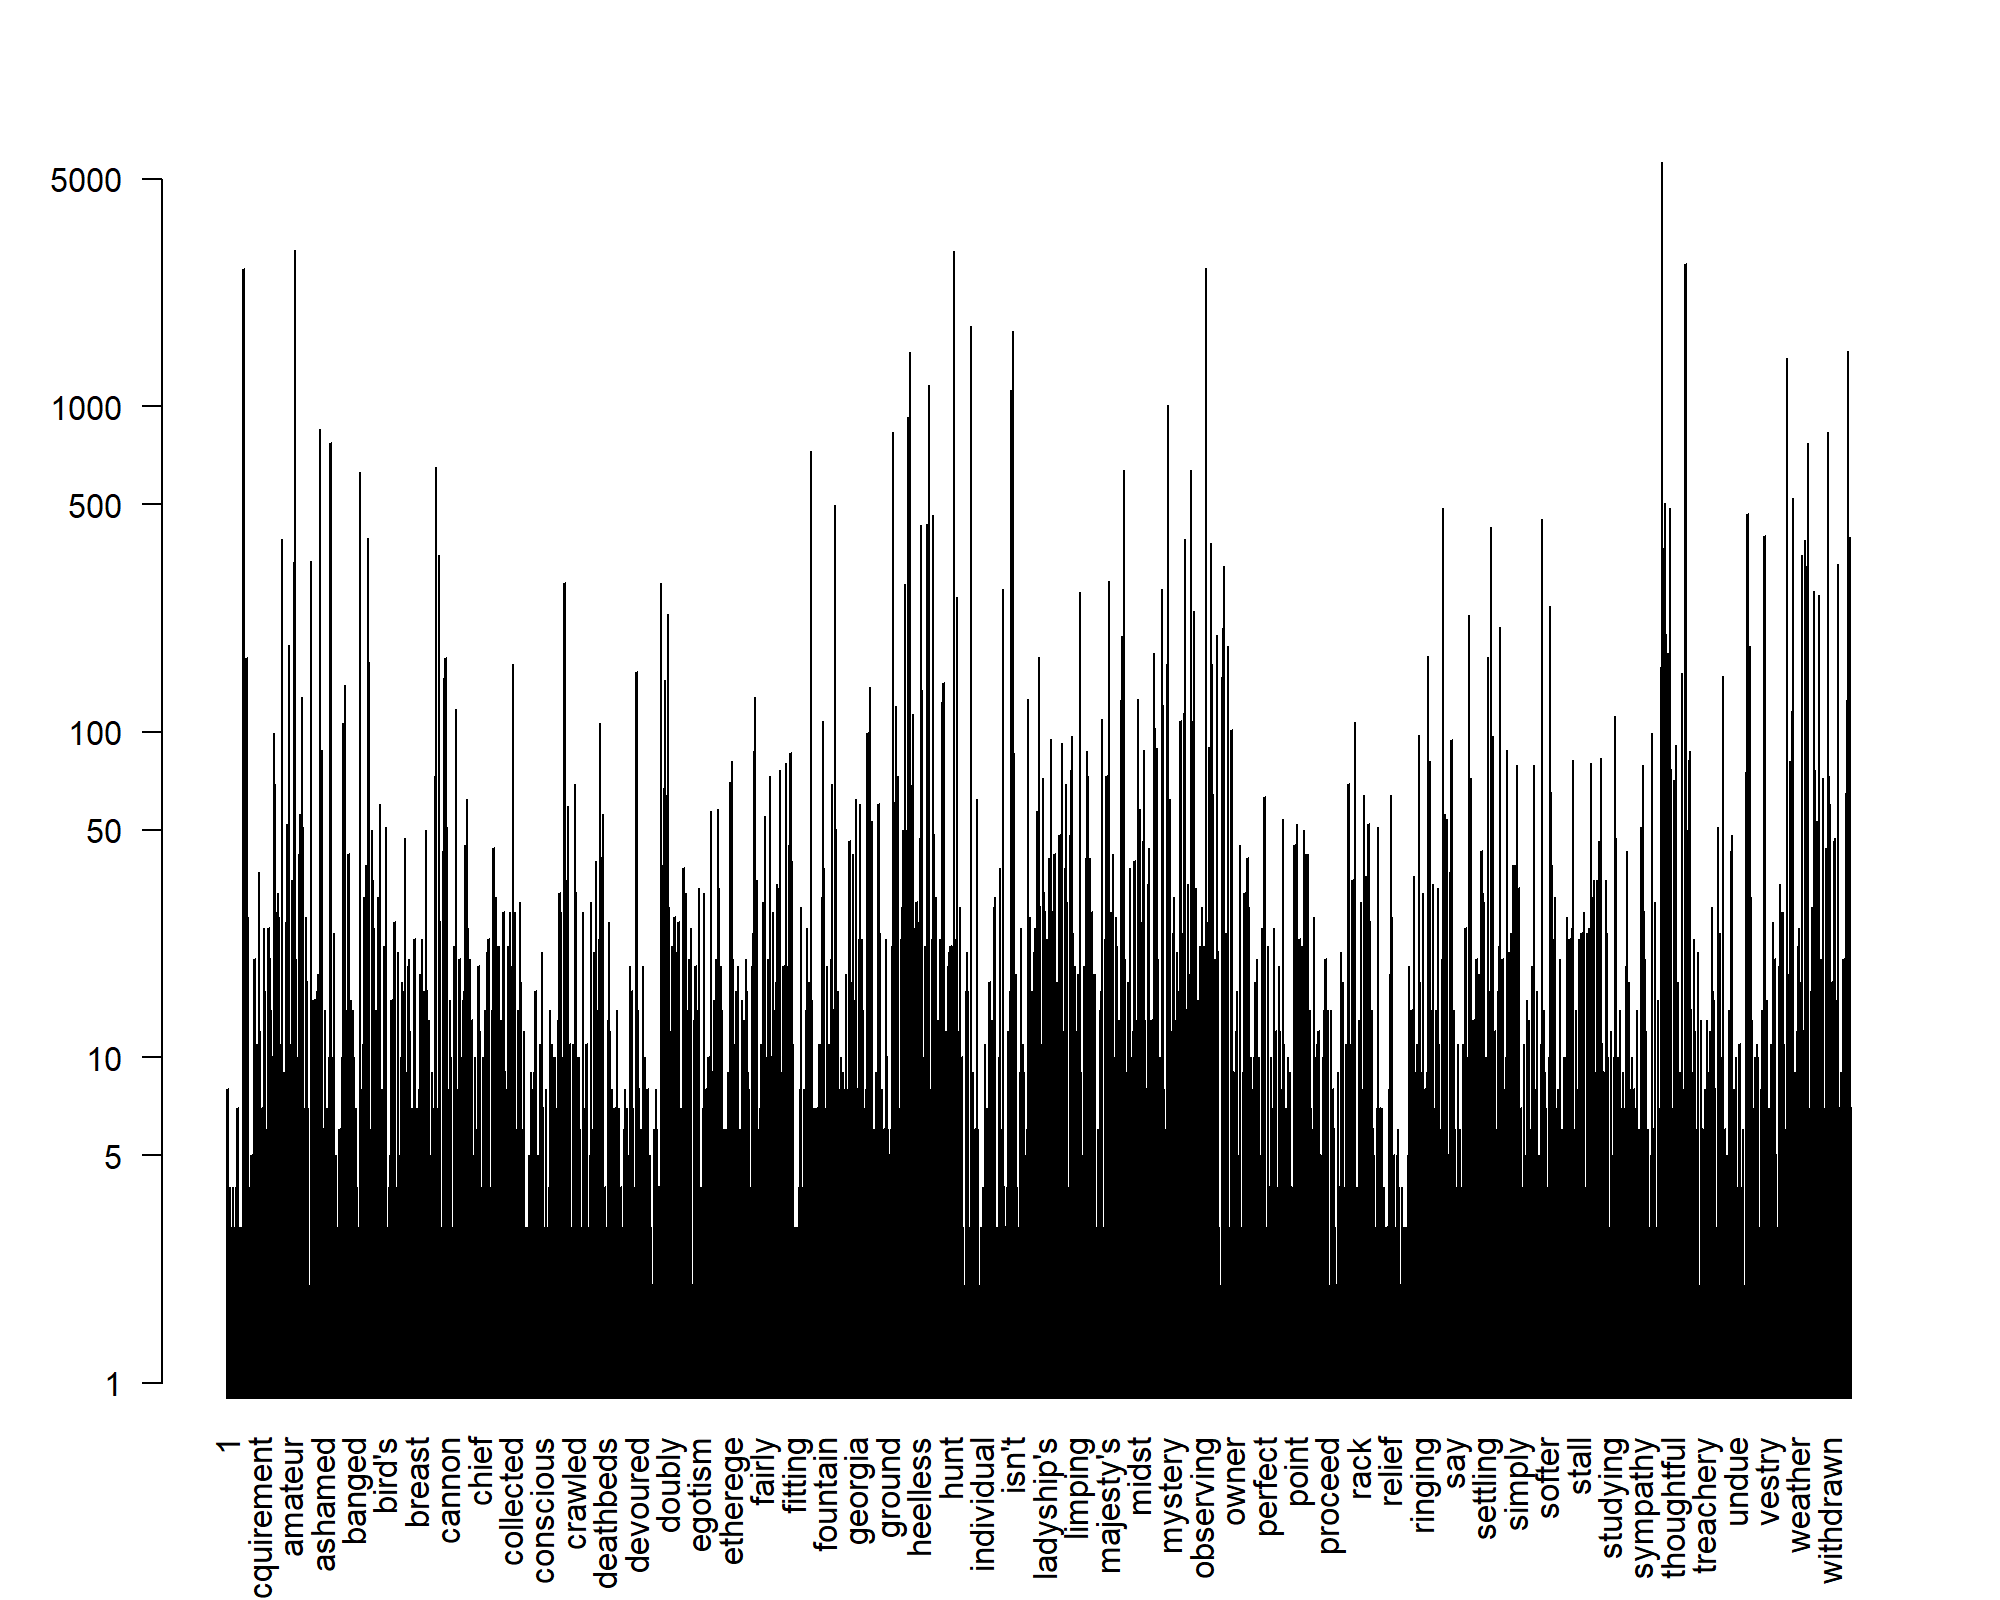
\includegraphics[scale=0.65]{figuras/frecuenciapalabra.png}
\caption{Histogramas de frecuencia de ocurrencia de las palabras en el texto en el texto, usando la escala logarítmica para mejor comprensión del gráfico}
\label{fig:2}
\end{figure}
\end{center}
 
Como se puede observar en la figura \ref{fig:2}, hay palabras que aparecen en pocas ocasiones en el texto y otras que se repiten gran cantidad de veces, estos extremos nos impiden hacer un análisis mas a fondo del contenido del texto, por lo que se realiza un filtrado de las palabras por frecuencia de ocurrencia tomando solamente aquellas que aparecen más de 200 y menos de 450 veces, el resultado de este filtro se muestra en el cuadro \ref{tab:5} de la página \pageref{tab:5} y gráficamente en la figura \ref{fig:3} de la página \pageref{fig:3} y en la nube de palabras que se muestra en la figura \ref{fig:4} de la página \pageref{fig:4}.

% Table generated by Excel2LaTeX from sheet 'Hoja1'
\begin{table}[htbp]
  \centering
  \caption{fragmento de \textit{Data frame} frecuencia de ocurrencia de las palabras en el texto en un rango de 200 -- 450 veces}
    \begin{tabular}{clc}
    \toprule
          & \textbf{Var1} & \multicolumn{1}{l}{\textbf{Freq}} \\
    \midrule
    274   & all   & 392 \\
    333   & an    & 332 \\
    417   & are   & 335 \\
    697   & been  & 393 \\
    1046  & by    & 349 \\
    1667  & could & 286 \\
    2143  & do    & 286 \\
    2177  & down  & 230 \\
    3350  & has   & 284 \\
    \bottomrule
    \end{tabular}%
  \label{tab:5}%
\end{table}%


\begin{center} 
\begin{figure}
\subfigure[Frecuencia de ocurrencia de las palabras en el texto en un rango de 200--450 veces ]{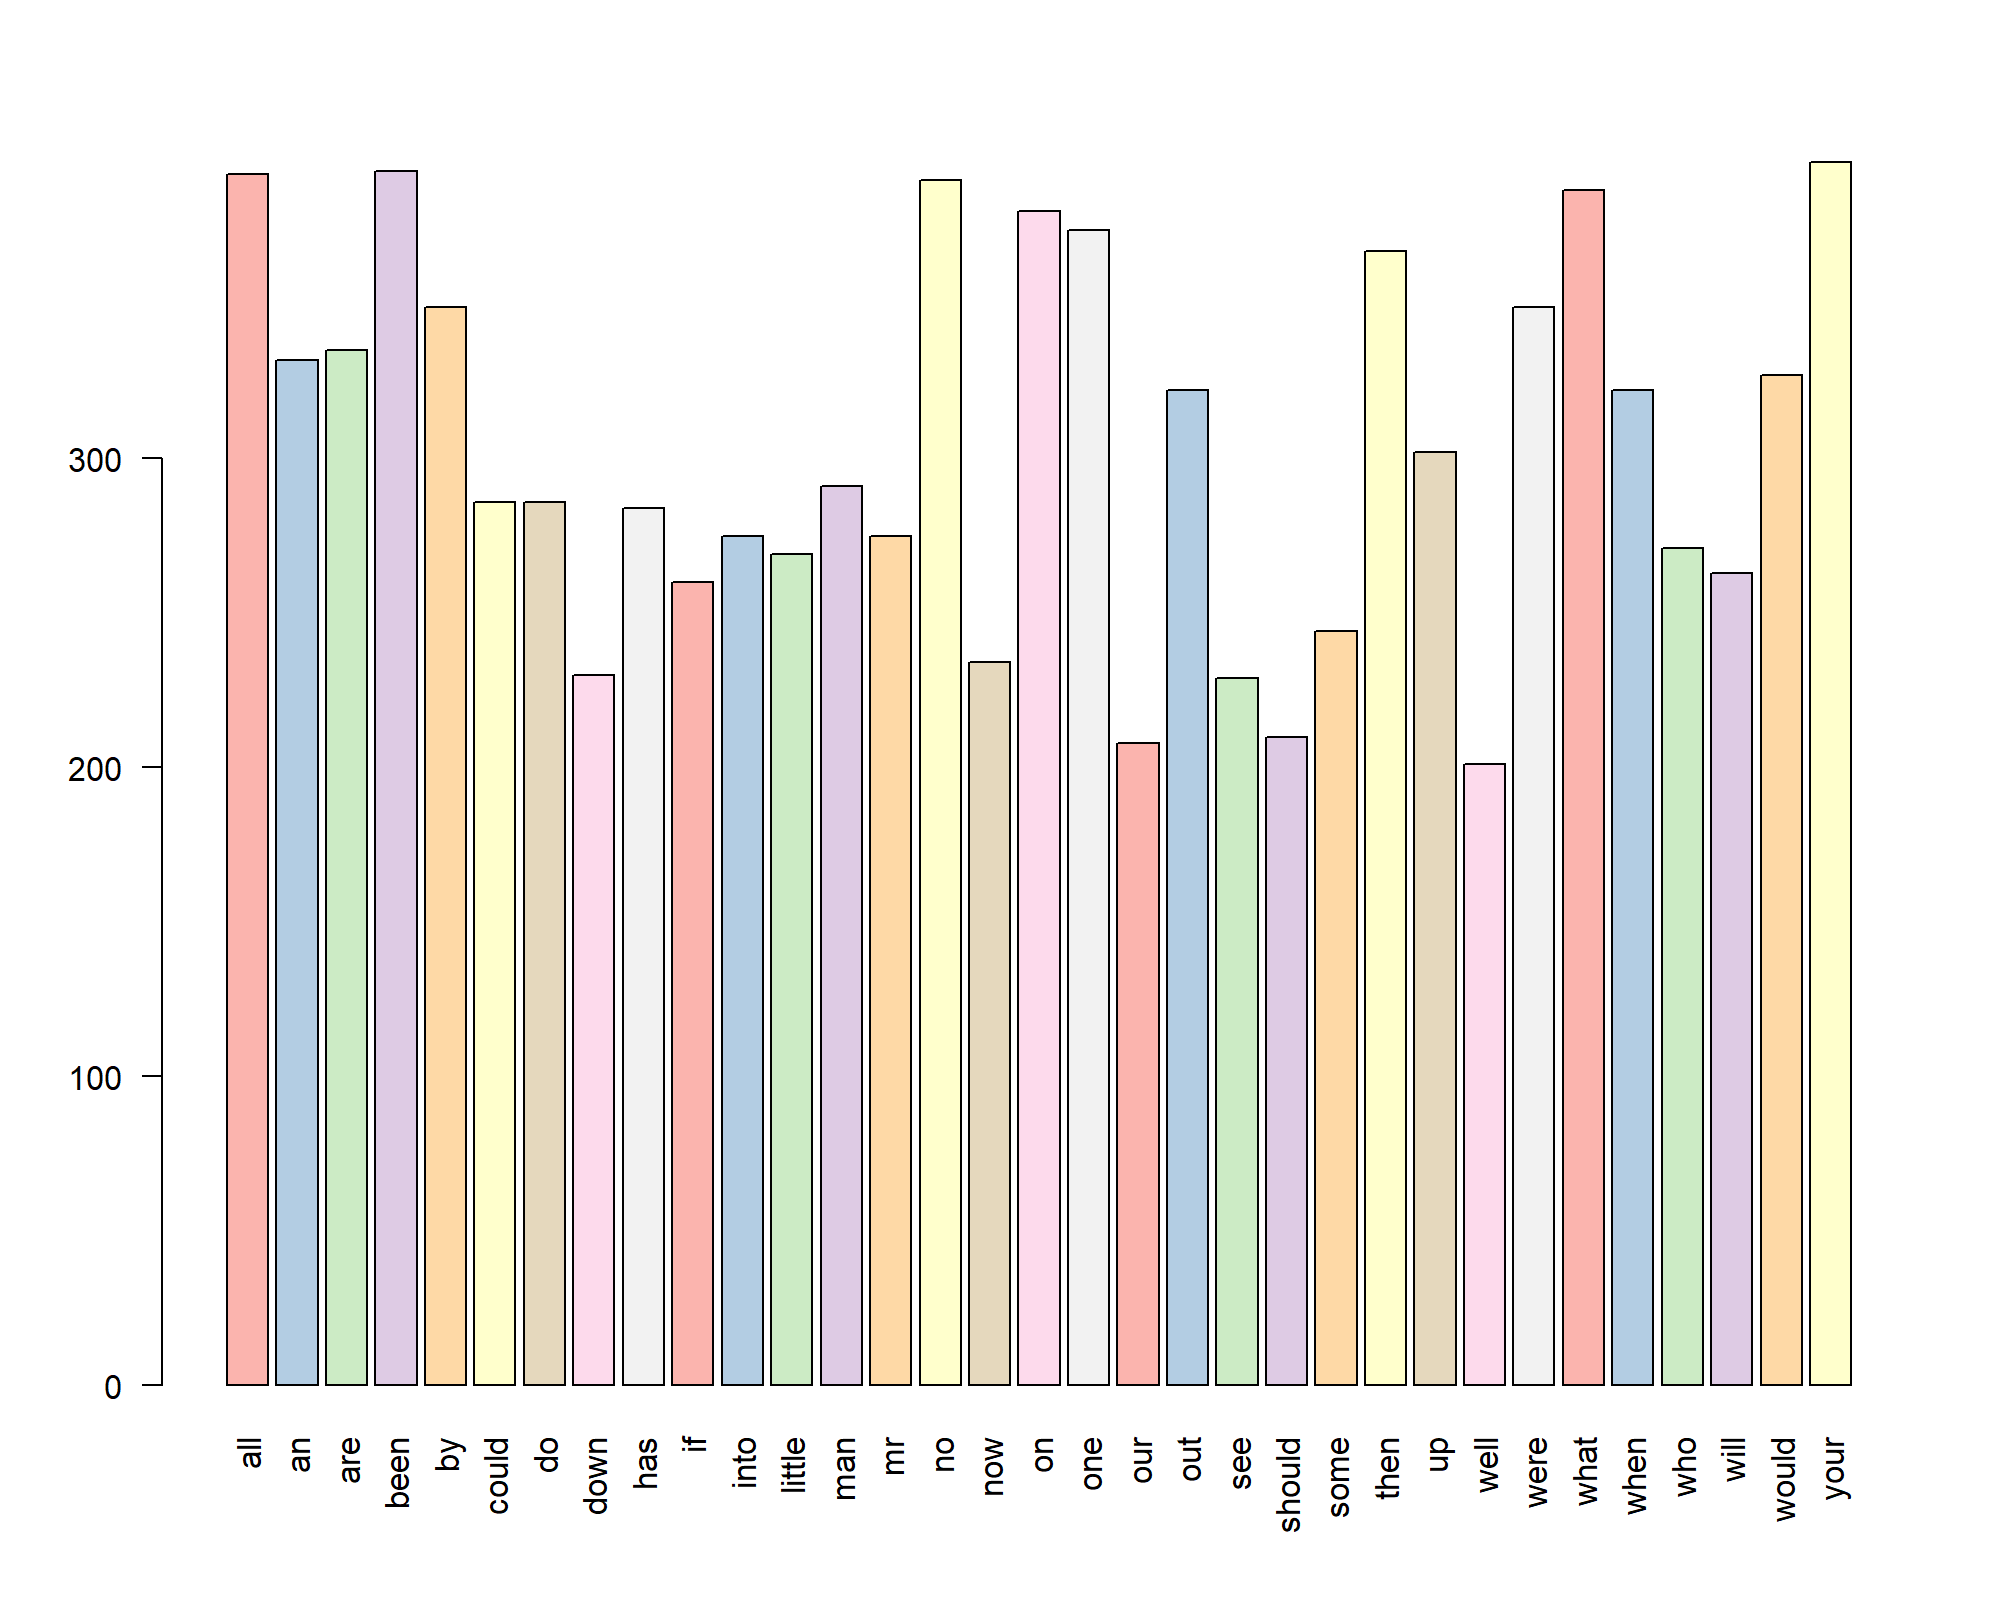
\includegraphics[scale=0.50]{figuras/frecuenciapalabrafiltro.png}}
\vspace{-0.3cm}
\subfigure[Frecuencia de ocurrencia de las palabras en el texto en un rango 200 -- 450 veces, ordenada de manera decreciente]{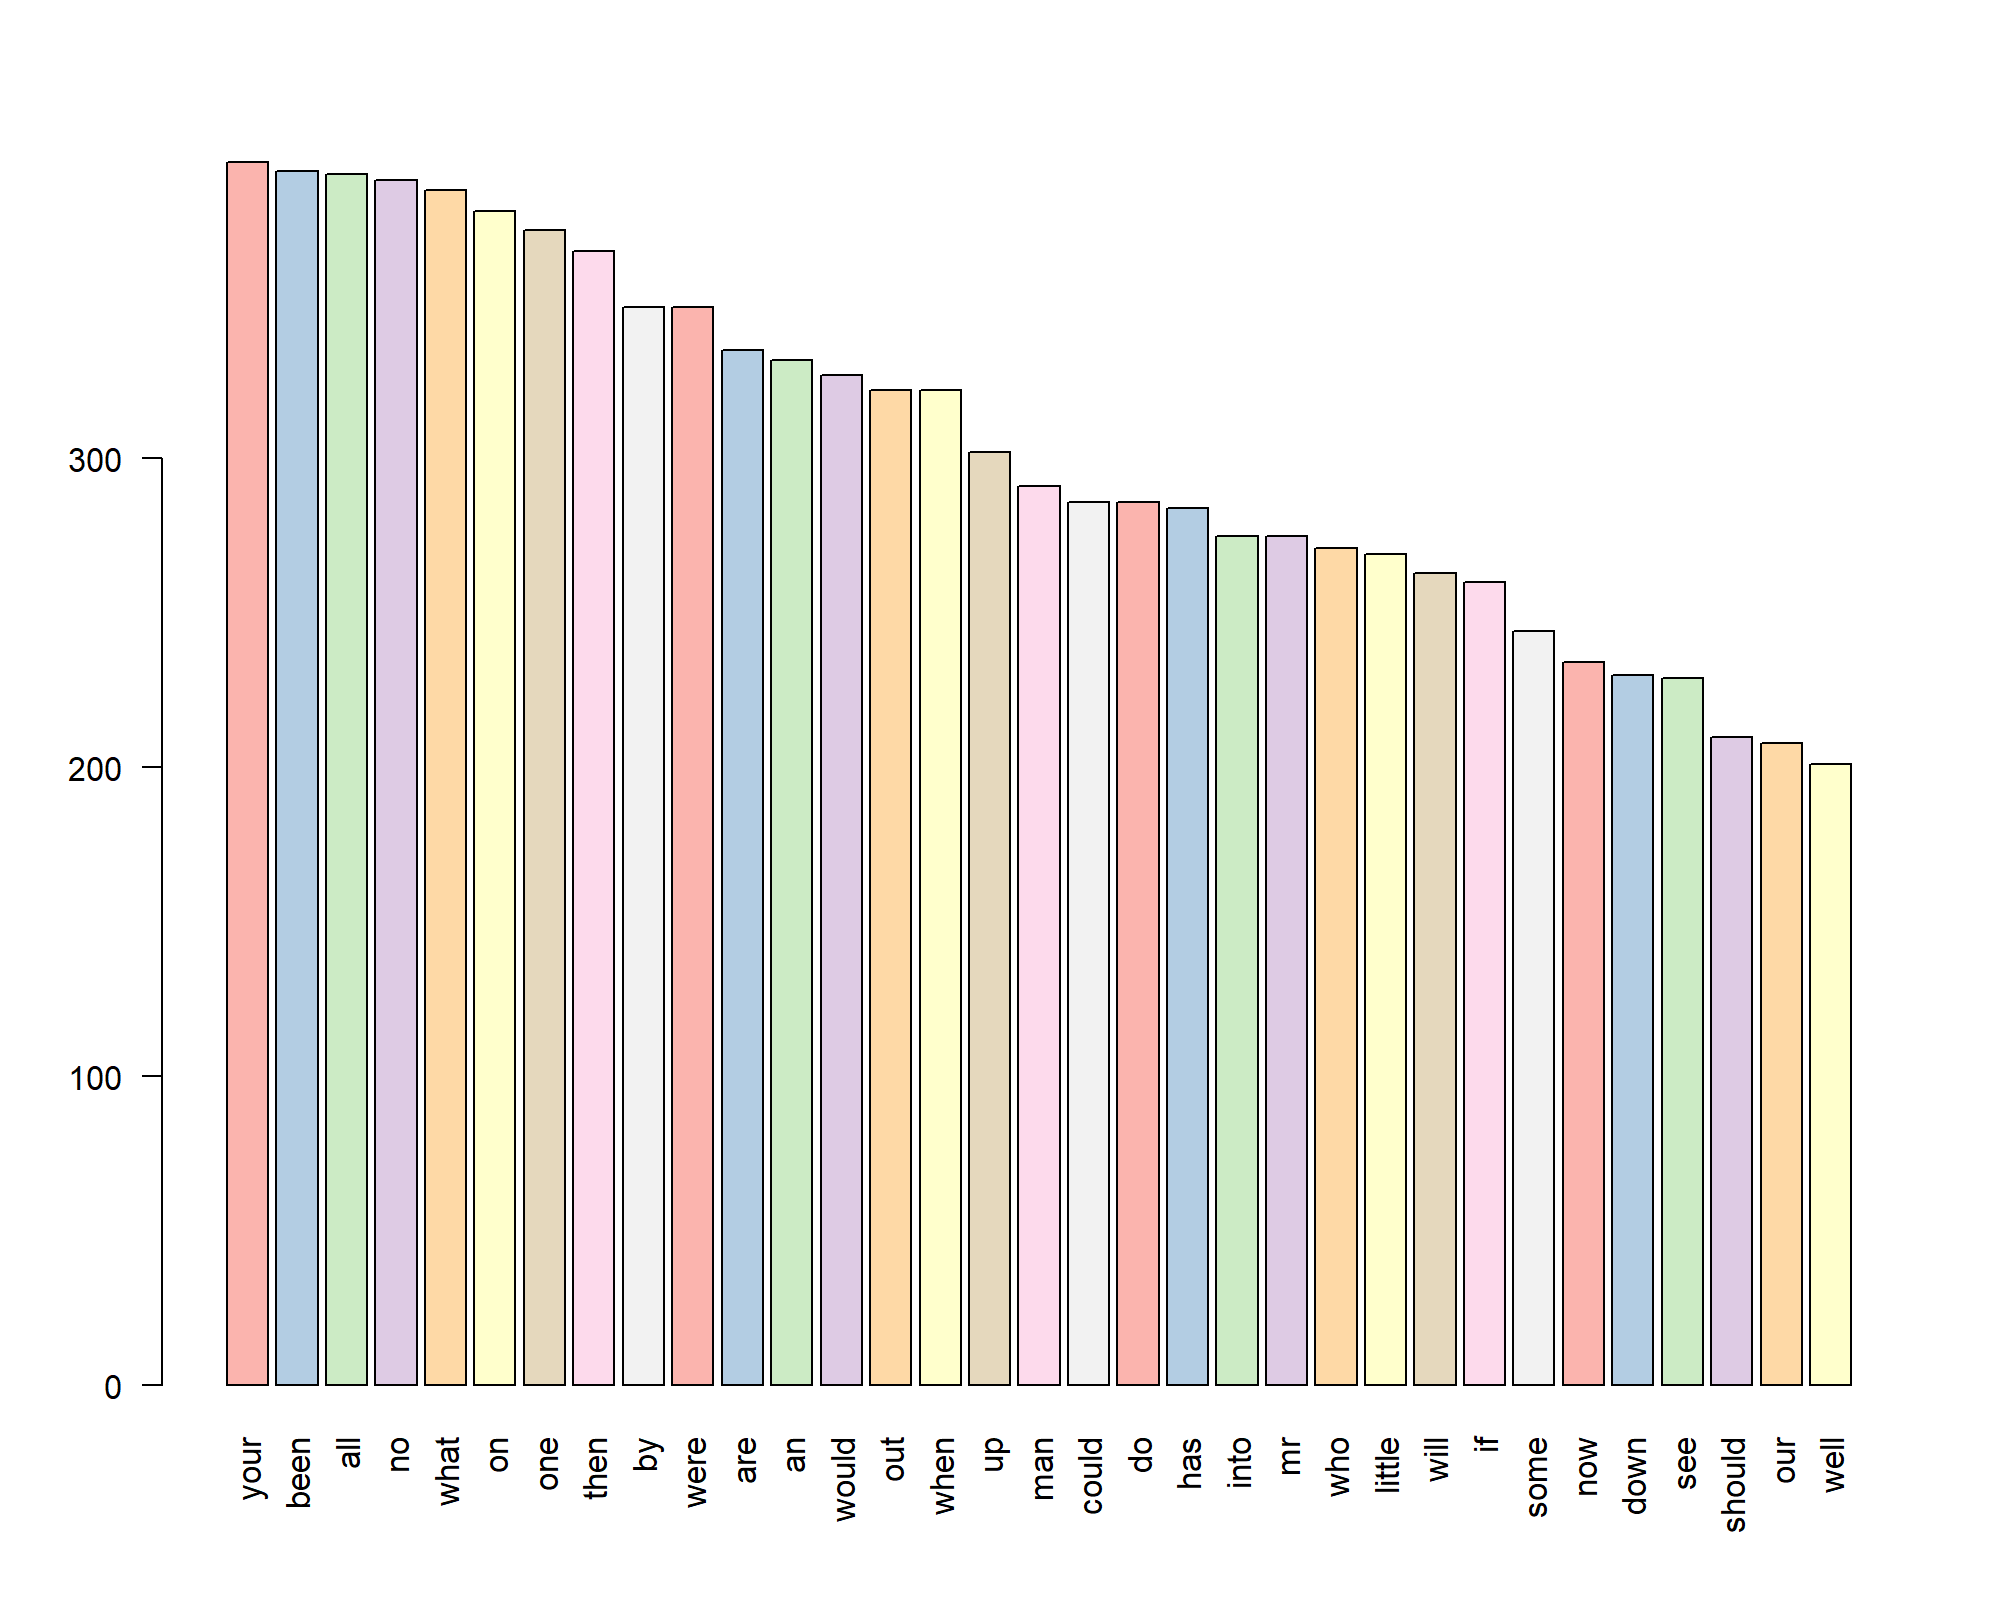
\includegraphics[scale=0.50]{figuras/frecuenciapalabrafiltroord.png}}
\caption{Frecuencia de ocurrencia de las palabras en el texto en un rango 200 -- 450 veces}
\label{fig:3} 
\end{figure}
\end{center}
 
 \begin{center}
\begin{figure}
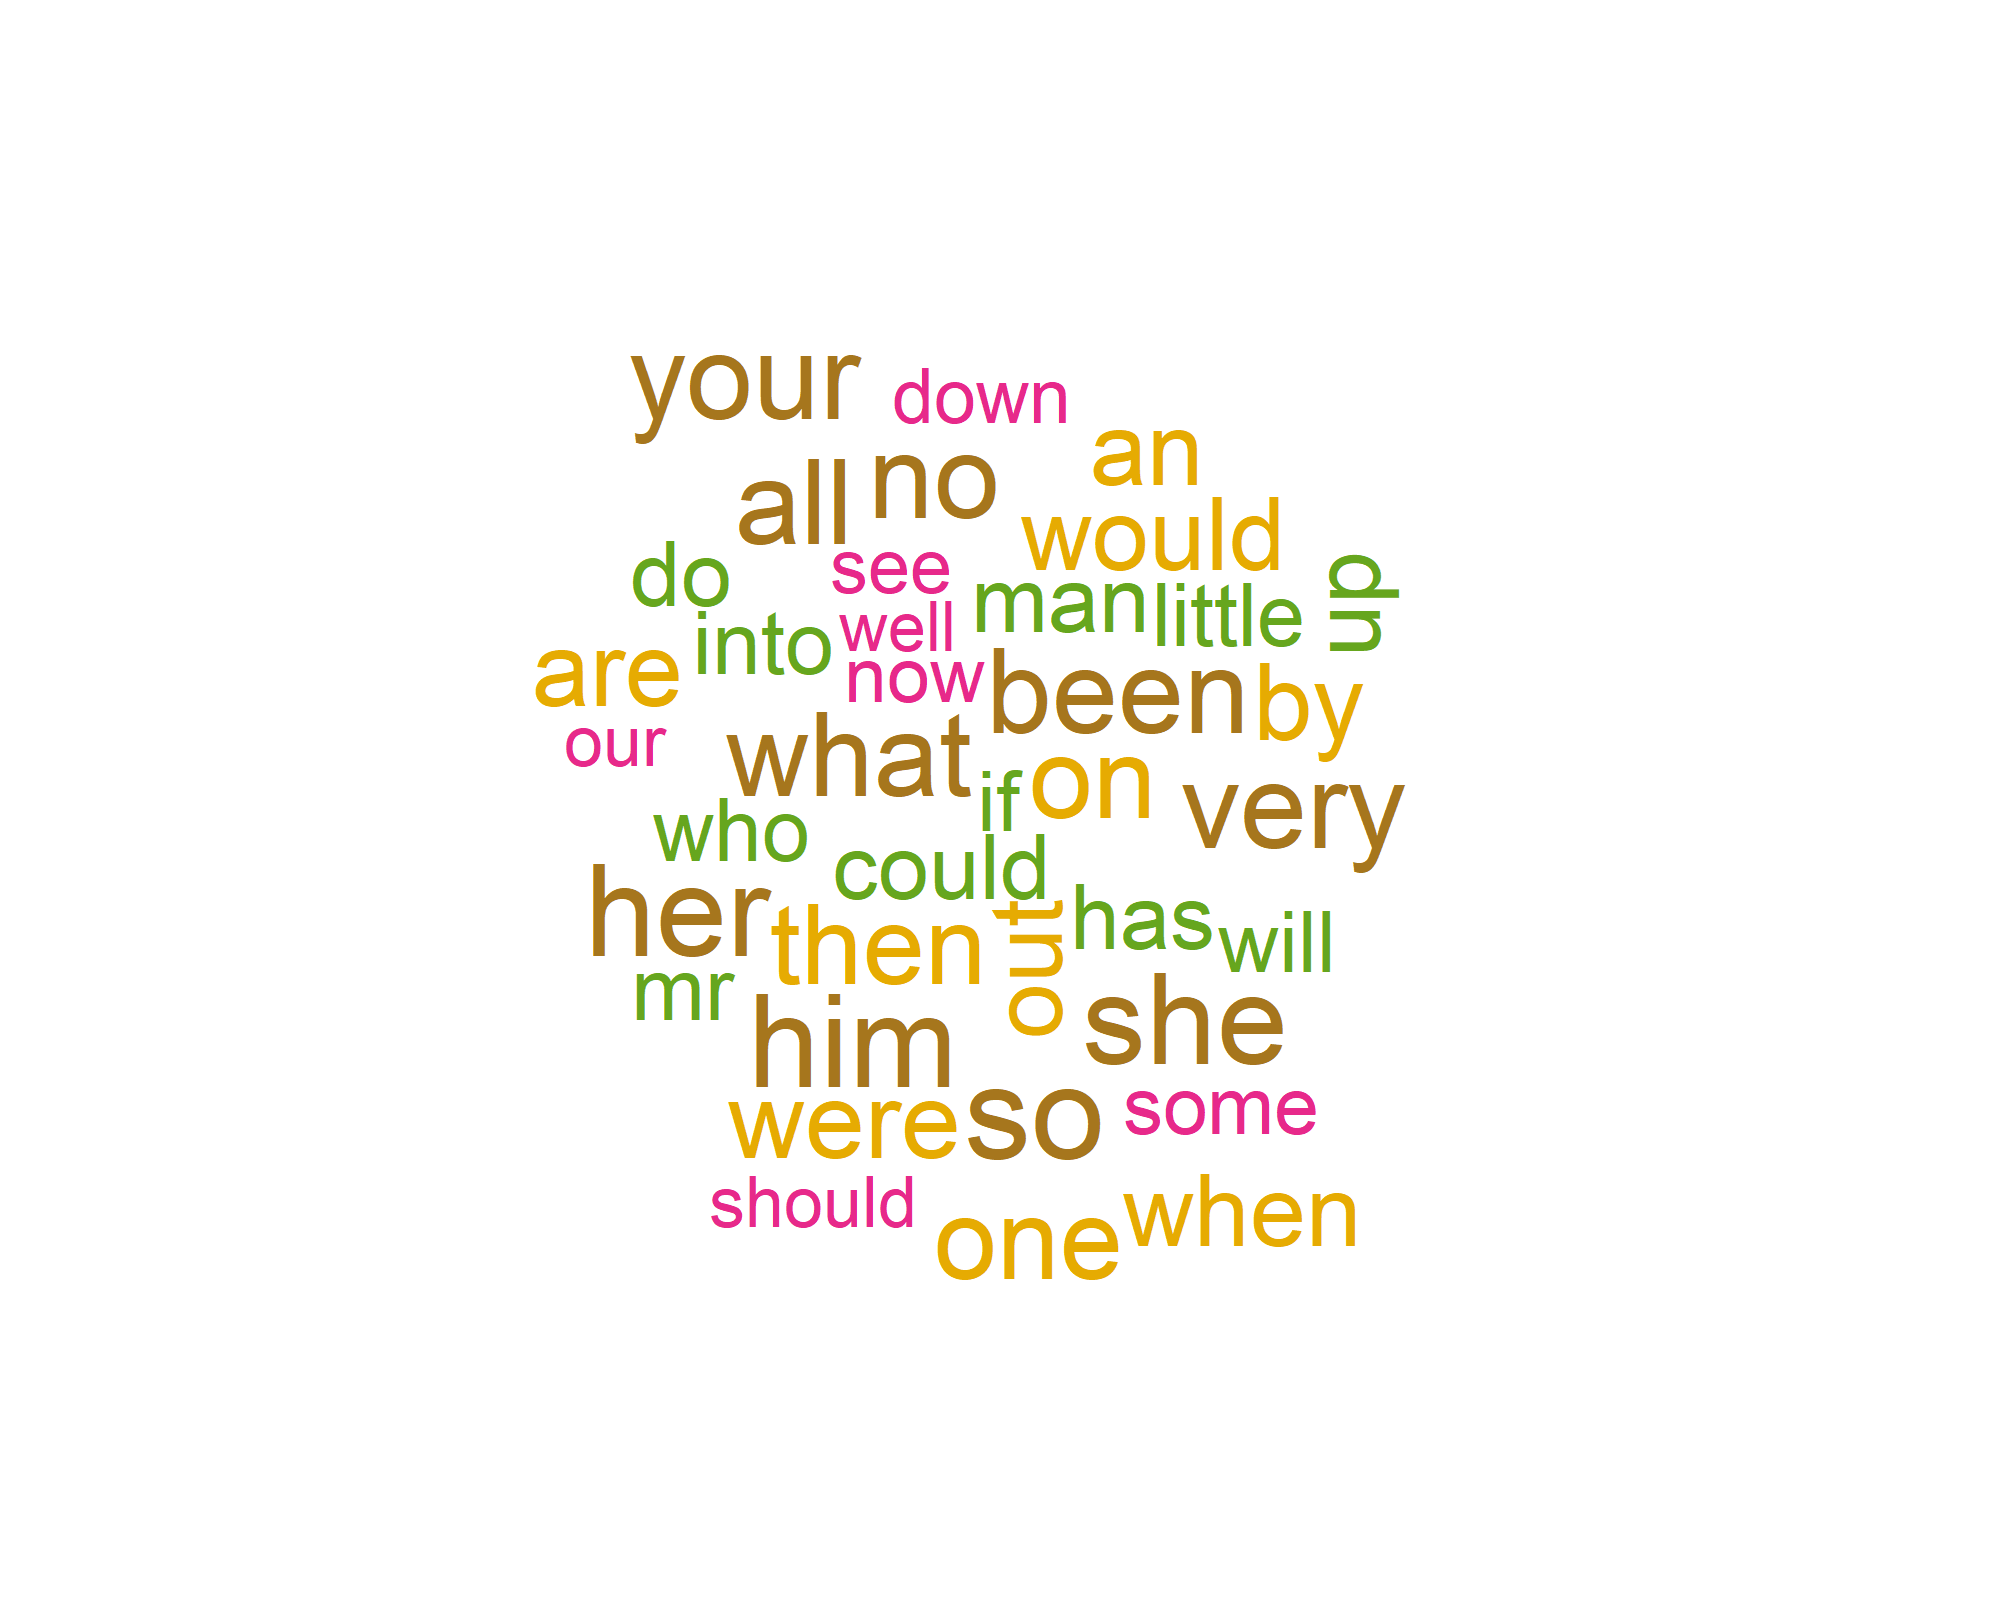
\includegraphics[scale=0.65]{figuras/nubedepalabras.png}
\caption{Nube de palabras utilizadas en el texto en un rango 200 -- 450}
\label{fig:4}
\end{figure}
\end{center}
 
 Además se analizan los pares de palabras que aparecen juntas en el texto, como se muestra en la figura \ref{fig:3} de la página \pageref{fig:3}

\begin{center}
\begin{figure}
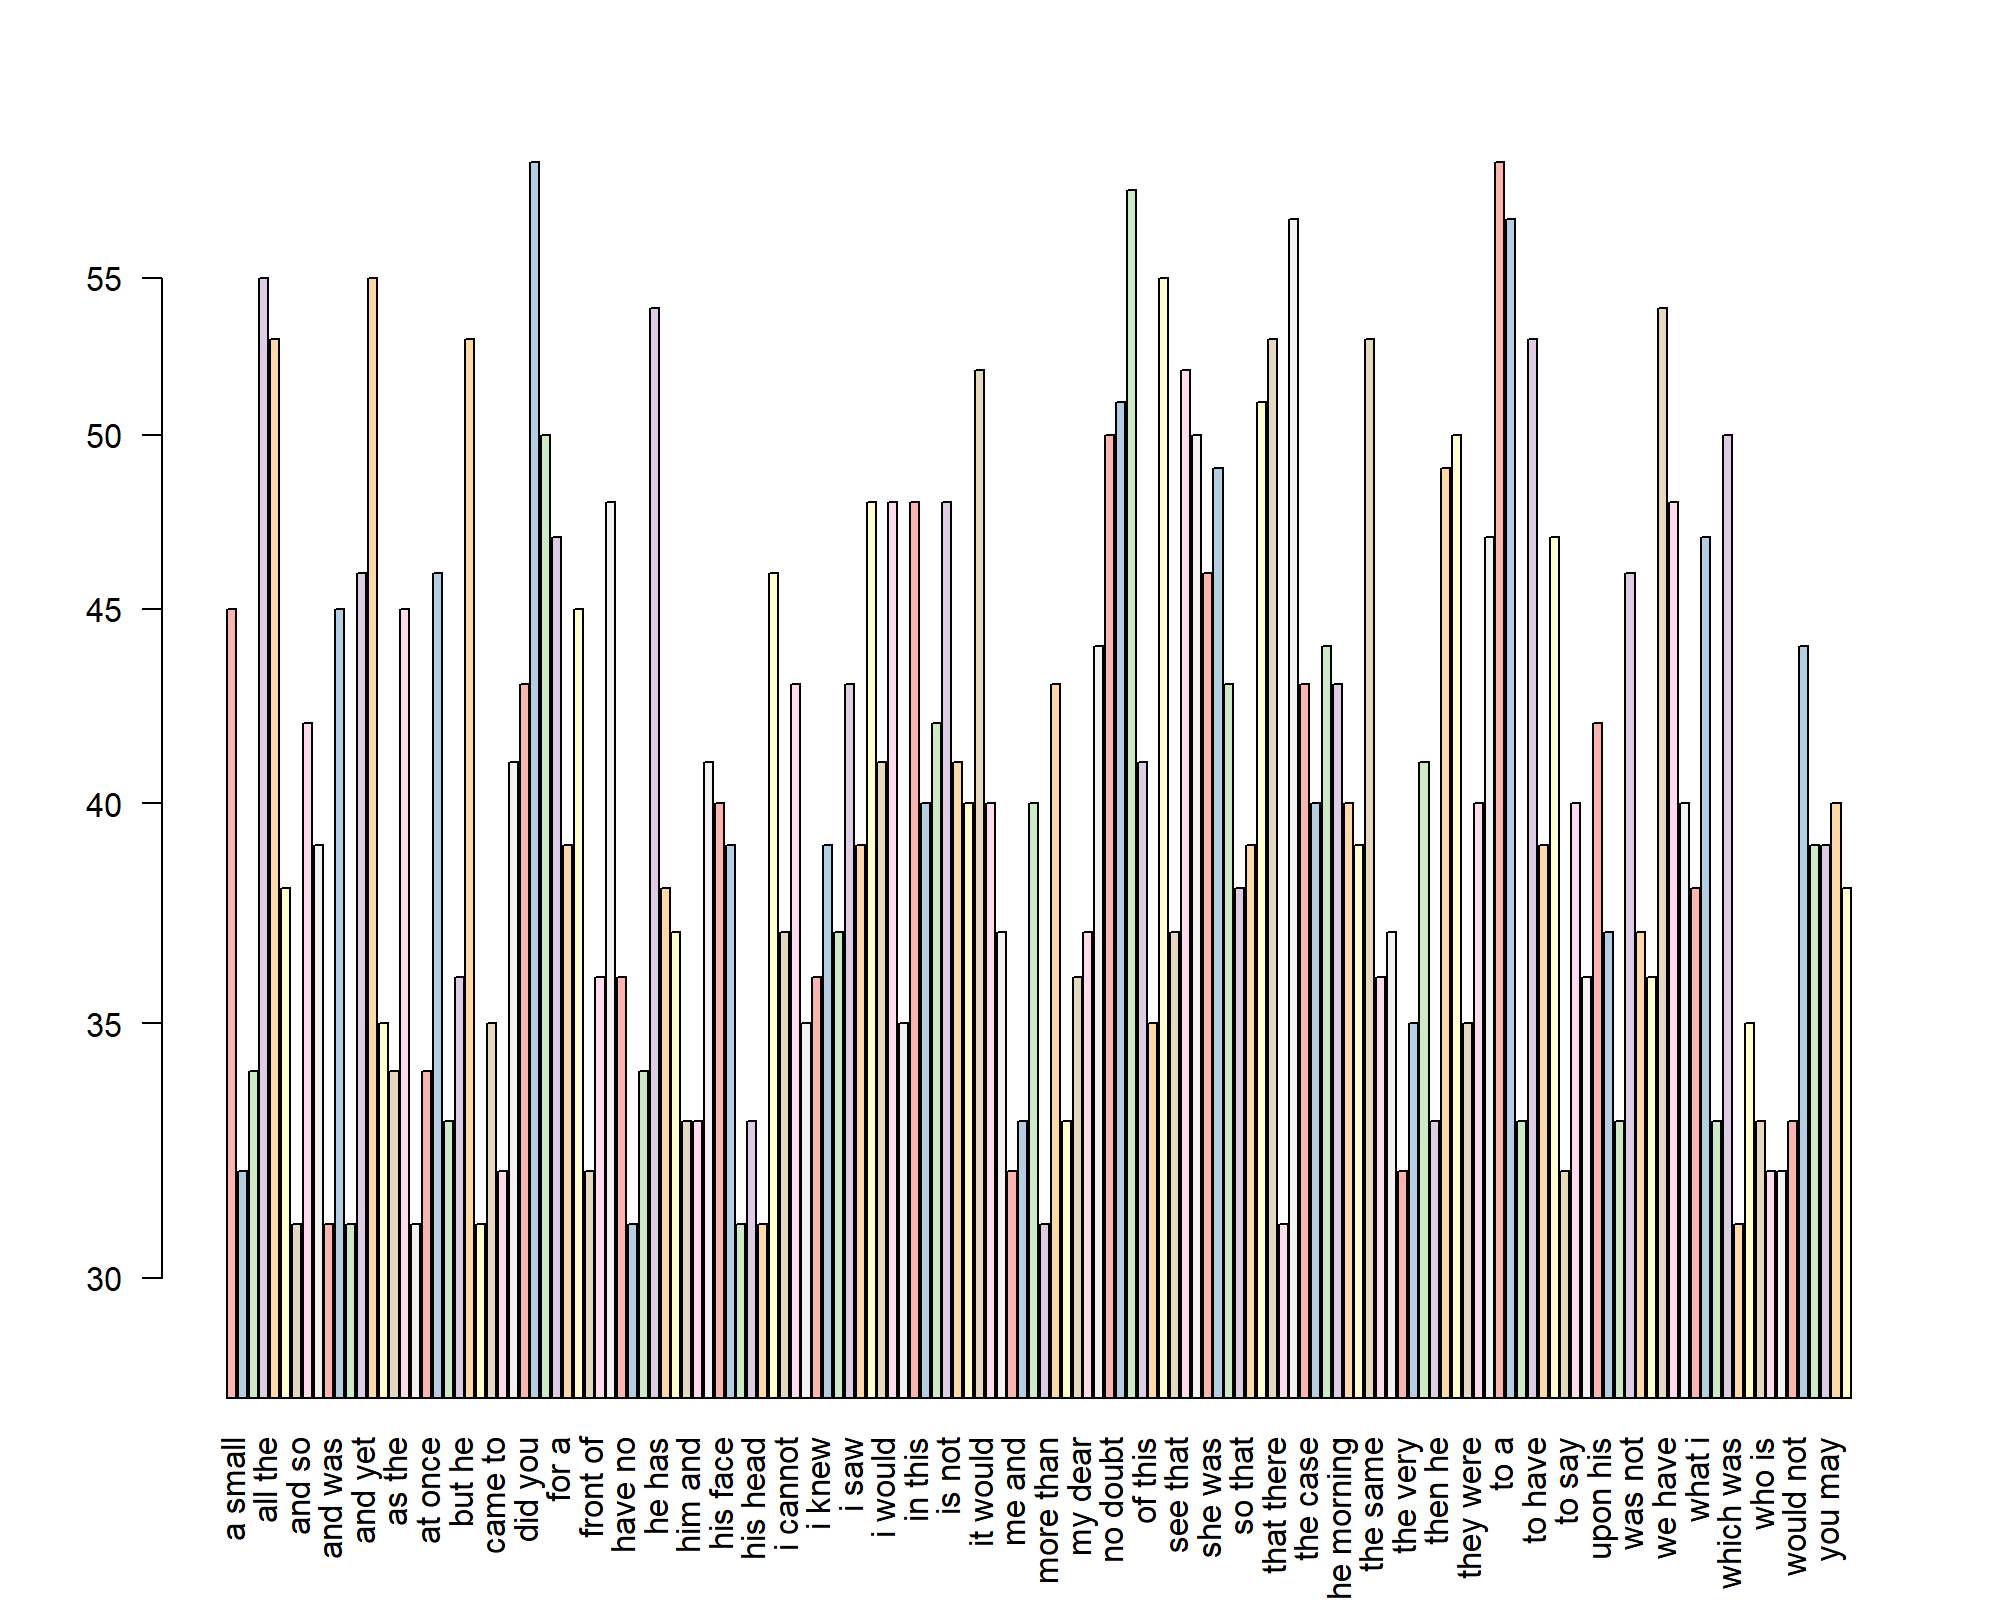
\includegraphics[scale=0.7]{figuras/ngrams.png}
\caption{histograma de pares de palabras usadas en el texto en un rango de 30 -- 60 veces}
\label{fig:5}
\end{figure}
\end{center}


El código general se encuentra disponible en el repositorio \href{https://github.com/Albertomnoa/Tareas_MPA/tree/master/Tarea2}{https://github.com/Albertomnoa/Tareas\_MPA/Tarea2} 

\newpage
\bibliographystyle{plain}
\bibliography{tarea1}

\end{document}
